\chapter{Aritmética del Computador y Fuentes de error}\label{chp:arit}
En el capítulo 1, introdujimos la representación binaria de números así como la conversión de binario a decimal y decimal a binario. A lo largo de este capítulo vamos a profundizar más en el modo en que el ordenador representa y opera con los números así como en una de sus consecuencias inmediatas: la imprecisión de los resultados. 

\section{Representación binaria y decimal}\index{Binario}

Los números reales pueden representarse empleando para ello una recta que se extiende entre $-\infty$ y $+\infty$. La mayoría de ellos no admiten una representación numérica exacta, puesto que poseen infinitos decimales. 

Los números enteros, $1, -1, 2, -2, 3, -3, \cdots$ admiten una representación numérica exacta. \index{Notación científica} En cualquier caso, rara vez manejamos números enteros con una cantidad grande de dígitos, habitualmente, los aproximamos, expresándolos en notación científica, multiplicándolos por una potencia de $10$. Tomemos un ejemplo de la química: la cantidad de átomos o moléculas que constituyen un mol de una sustancia se expresa por el número de Avogadro, $N_A=6.02214179 \times 10^{23}$, dicho numero, --que debería ser un entero--  se expresa empleando tan solo 9 de sus 23 cifras significativas (a veces tan solo se dan las tres primeras). 

\index{Truncamiento} Cuando truncamos un número, es decir, despreciamos todos sus dígitos hacia la derecha a partir de uno dado, estamos aproximando dicho número por un  número racional, es decir, por un número que puede expresarse como el cociente entre dos números enteros. $1/2, 3/4, \cdots$ 

Algunos números racionales se reducen a su vez a números enteros, $6/3$, otros dan lugar a números cuya representación exige un número finito de dígitos: 
\begin{equation*}
11/2=(5.5)_{10}=5\times10^0+5\times10^{-1}
\end{equation*} 
Si representamos el mismo número en base 2 obtenemos,
\begin{equation*}
11/2=(101.1)_2=1\times2^2+0\times2^1+1\times2^0+1\times2^{-1}
\end{equation*}
Sin embargo, el que un número racional admita una representación finita, depende de la base en que se representa. Por ejemplo: $1/10=(0.1)_{10}$ no admite representación finita en base 2.
\begin{equation*}
1/10=(0.0001100110011\cdots)_2 =1\times2^{-4}+1\times2^{-5}+0\times2^{-6}+0\times2^{-7}+1\times2^{-8}+\cdots 
\end{equation*}
 
En este último caso, se trata de una representación que, aunque no termina, es repetitiva o periódica; tras el primer cero decimal se repite indefinidamente la secuencia: $0011$. Los números racionales admiten siempre una representación finita ó infinita periódica. 

El número racional $1/3=(0.333\cdots)_{10}=(0.010101\cdots)_2$ solo admite representación infinita periódica tanto en base 10 como en base 2. Sin embargo, admite representación finita si lo representamos en base 3: $1/3=(0.1)_3=0\times3^0+1\times3^{-1}$.

Habitualmente, en la vida ordinaria, representamos los números en base 10, sin embargo, como hemos visto en el capítulo 1 el ordenador emplea una representación binaria. Como acabamos de ver, una primera consecuencia de esta diferencia, es que al pasar números de una representación a otra estemos alterando la precisión con la que manejamos dichos números. Esta diferencia de representación supone ya una primera fuente de errores, que es preciso tener en cuenta cuando lo que se pretende es hacer cálculo científico con un ordenador. Como iremos viendo a lo largo de este capítulo, no será la única.

\section{Representación de números en el ordenador}\index{Representación numérica}
\paragraph{Enteros positivos} La forma mas fácil de representar números sería empleando directamente los registros de memoria para guardar números en binario.  Si suponemos un ordenador que tenga regis-\- tros de 16 bits. Podríamos guardar en ellos números comprendidos entre el $0$ y el $2^{16}-1=65535$. Este último se representaría con un $1$ en cada una de las posiciones del registro, en total 16 unos. Se trata del entero más grande que podríamos representar con un registro de 16 bits:
\\

\begin{tabular}{|l|c|c|c|c|c|c|c|c|c|c|c|c|c|c|c|c|}
\hline
posición&1&2&3&4&5&6&7&8&9&10&11&12&13&14&15&16  \\
\hline
valor&1&1&1&1&1&1&1&1&1&1&1&1&1&1&1&1 \\
\hline
\end{tabular}\\

 Hasta ahora, nuestro sistema de representación solo admite números enteros. El menor número que podemos representar es el cero, y el mayor ---dependerá del tamaño $n$ de los registros del ordenador---, $2^n-1$.  Es evidente que este sistema de representación resulta insuficiente.
 
 \paragraph{Enteros positivos y negativos}
 Un primera mejora consistiría en ampliar el sistema de representación para que admita también números negativos. Una posibilidad sería reservar uno de los bits del array para representar el signo \index{Bit de signo}, y usar los restantes para representar el número. En nuestro ejemplo de un registro de 16 bits, el número más grande sería ahora $2^{15}-1$ y el más pequeño sería $-2^{15}+1$. El cero tendría una doble representación, una de ellas con signo más y la otra con signo menos.
 
 Una representación alternativa, cuyo uso está muy extendido en las máquinas, es la representación conocida con el nombre de \emph{Complemento a 2} \index{Complemento a dos} \index{Representación numérica!}. Supongamos un registro de n bits:
 \begin{itemize}
 \item Un entero $x$ no negativo se almacena empleando directamente su representación binaria. el intervalo de enteros no negativos representables es: $0 \le x \le 2^{(n-1)}-1$.
 \item Un entero negativo $-x$, donde $1 \le x \le 2^{(n-1)}$, se almacena como la representación binaria del entero positivo: $2^{n}-x$
 \item El número así construido,  recibe el nombre de complemento a 2 de x.
 \end{itemize}
 En general, dado un número entero $N<2^n$ su complemento a dos en una representación binaria de $n$ dígitos se define como:
 \begin{equation*}
 C_2^N=2^n-N
 \end{equation*} 
 Veamos un ejemplo de esta representación, para el caso de un registro de 4 bits:
 
 \begin{table}
 \centering
 \begin{tabular}{r  l  r  r}
 Decimal&  (4 bits) &\ $C_2=2^n-x$ & n. representado\\
 \hline
15& 1111&$(16-1)=15$&-1\\
14& 1110&$(16-2)=14$&-2\\
13& 1101&$(16-3)=13$&-3\\
12& 1100&$(16-4)=12$&-4\\
11& 1011&$(16-5)=11$&-5\\
10& 1010&$(16-6)=10$&-6\\
9& 1001& $(16- 7)=9$&-7\\
8& 1000& $(16-8)=8$&-8\\
\hline
\hline
7& 0111& & 7\\
6& 0110& & 6\\
5& 0101& & 5\\
4& 0100& & 4\\
3& 0011& & 3\\
2& 0010& & 2\\
1& 0001& & 1\\
0& 0000& & 0\\
\hline
\end{tabular}
 \end{table}
 

 La representación en complemento a 2 tiene las siguientes características:
 \begin{itemize}
 \item La representación de los números positivos coincide con su valor binario
 \item La representación del número 0 es única.
 \item El rango de valores representables en una representación de N bits es $-2^{N-1} \le x \le  2^{N-1}-1$.
 \item Los números negativos se obtienen como el complemento a dos, cambiado de signo,  del valor binario que los representa. 
 \end{itemize}

Una forma práctica de obtener el complemento a dos de un número binario es copiar el número original de  derecha a izquierda hasta que aparezca el primer 1. Luego de copiar el primer 1, se complementan el resto de los bits del número (si es 0 se pone un 1 y si es 1 se pone un 0). Por ejemplo el complemento a dos del número 2, (0010 en una representación de 4 bits) sería 1110,

\begin{eqnarray*}
001\mathbf{0} & \xrightarrow{copia\  bit\ derecha }& \cdots 0 \\
00\mathbf{1}0 & \xrightarrow{copia\ primer\ bit = 1}& \cdot \cdot 10\\ 
0 \mathbf{0}10& \xrightarrow{complemento\ bit\  0} &\cdot  \ 110\\
 \mathbf{0}010& \xrightarrow{complemento\ bit\ 0} &1110
\end{eqnarray*} 

\index{Complemento a dos! Sustracción} Una propiedad importante de la representación de complemento a dos, es que la diferencia de dos números puede realizarse directamente sumando al primero el complemento a dos del segundo. Para verlo podemos usar los dos números del ejemplo anterior: $0010$ es la representación binaria del número $2$, si empleamos un registro de cuatro bits. Su complemento a dos, $1110$ representa al número $-2$. Si los sumamos \index{Adición en binario} \footnote{Sumar en binario es como sumar en decimal. Se procede de bit a bit, de derecha a izquierda y cuando se suman 1 y 1, el resultado es 10 (base 2), de modo que el bit resultante se coloca en 0 y se lleva el 1 hacia el siguiente bit de la izquierda.}:

\begin{table}
 \centering
\begin{tabular}{|c|c|c|c|c|}
\hline
 &0&0&1&0\\
 \hline
  &1&1&1&0\\
  \hline
  \textbf{1}&0&0&0&0\\
  \hline
  \hline
  &0&0&0&0\\
  \hline
\end{tabular}
\end{table}

El resultado de la suma nos da un número cuyos primeros cuatro bits son 0. El bit distinto de cero, no puede ser almacenado en un registro de cuatro bits, se dice que el resultado de la operación \emph{desborda} el tamaño del registro. Ese bit que no puede almacenarse se descarta al realizar la operación de suma, con lo que el resultado sería cero, como corresponde a la suma de $2+(-2)$. Esta es la motivación fundamental para emplear una representación en complemente a dos: No hace falta emplear circuitos especiales para calcular la diferencia entre dos números, ya que ésta se representa como la suma del minuendo con el complemento a dos del sustraendo.

\subsection{Números no enteros: Representación en punto fijo y en punto flotante}
La representación de números no enteros se emplea para representar de modo aproximado números reales. Como hemos dicho antes, los números racionales periódicos y los números irracionales no pueden representarse de forma exacta mediante un número finito de decimales. Por esta razón, su representación es siempre aproximada. Para los números racionales no periódicos, la representación será exacta o aproximada dependiendo del número que se trate, el tamaño de los registros del ordenador y el sistema empleado para la representación. Los dos sistemas de representación más conocidos son la representación en  punto fijo y, de especial interés para el cálculo científico, la representación en punto flotante.

\paragraph*{Representación en punto fijo.} \index{Representación numérica! en punto fijo}En la representación en punto fijo, el registro empleado para almacenar un número se divide en tres partes: 
\begin{itemize}
\item 1 bit para almacenar el signo del número.  
\item Un campo de bits de tamaño fijo para representar la parte entera del número.
\item Un campo para almacenar la parte decimal del número
\end{itemize}

Por ejemplo, si tenemos un registro de 16 bits podemos reservar 1 bit para el signo, 7 para la parte entera y 8 para la parte decimal.  La representación en punto fijo del número binario $-10111.0011101101$ sería: \\


\begin{tabular}{|c||c|c|c|c|c|c|c||c|c|c|c|c|c|c|c|}
\hline
s&\multicolumn{7}{c||}{p. entera}&\multicolumn{8}{c|}{p. decimal}\\
\hline
1&0&0&1&0&1&1&1&0&0&1&1&1&0&1&1\\
\hline
\end{tabular}\\

Es interesante notar cómo para representar la parten entera, nos sobran dos bits en el registro, ya que la parte entera solo tiene cinco cifras y tenemos 7 bits para representarla. Sin embargo, la parte decimal tiene 10 cifras; como solo tenemos 8 bits para representar la parte decimal, la representación trunca el número eliminando los dos últimos decimales.

Si asociamos cada bit con una potencia de dos, en orden creciente de derecha a izquierda, podemos convertir directamente el número representado de binario a decimal,\\ 

\begin{tabular}{|c||c|c|c|c|c|c|c||c|c|c|c|c|c|c|c|}
\hline
s&\multicolumn{7}{c||}{p. entera}&\multicolumn{8}{c|}{p. decimal}\\
\hline
1&0&0&1&0&1&1&1&0&0&1&1&1&0&1&1\\
\hline
-&$2^{6}$&$2^{5}$&$2^{4}$&$2^{3}$&$2^{2}$&$2^{1}$&$2^{0}$&$2^{-1}$&$2^{-2}$&$2^{-3}$&$2^{-4}$&$2^{-5}$&$2^{-6}$&$2^{-7}$&$2^{-8}$\\
\hline
\end{tabular}\\

Por tanto el número representado sería,

\begin{equation*}
\begin{split}
&-(0\cdot 2^6+0 \cdot 2^5+ 1\cdot 2^4+ 0 \cdot 2^3+ 1 \cdot 2^2 + 1 \cdot 2^1 + 1 \cdot 2^0 + 0 \cdot 2^{-1}+ 0 \cdot 2^{-2}+ 1 \cdot 2^{-3}+ 1 \cdot 2^{-4}+ \\
& +1 \cdot 2^{-5}+0 \cdot 2^{-6} +1 \cdot 2^{-7}+1 \cdot {-8}) = - 23.23046875
\end{split}
\end{equation*}

De modo análogo podemos calcular cual sería el número más grande representable,\\

\begin{tabular}{|c||c|c|c|c|c|c|c||c|c|c|c|c|c|c|c|}
\hline
s&\multicolumn{7}{c||}{p. entera}&\multicolumn{8}{c|}{p. decimal}\\
\hline
0&1&1&1&1&1&1&1&1&1&1&1&1&1&1&1\\
\hline
&$2^{6}$&$2^{5}$&$2^{4}$&$2^{3}$&$2^{2}$&$2^{1}$&$2^{0}$&$2^{-1}$&$2^{-2}$&$2^{-3}$&$2^{-4}$&$2^{-5}$&$2^{-6}$&$2^{-7}$&$2^{-8}$\\
\hline
\end{tabular}\\

\begin{equation*}
\begin{split}
&1\cdot 2^6+1 \cdot 2^5+ 1\cdot 2^4+ 1 \cdot 2^3+ 1 \cdot 2^2 + 1 \cdot 2^1 + 1 \cdot 2^0 + 1 \cdot 2^{-1}+ 1 \cdot 2^{-2}+ 1 \cdot 2^{-3}+ 1 \cdot 2^{-4}+ \\
&+1 \cdot 2^{-5}+1 \cdot 2^{-6} +1 \cdot 2^{-7}+ 1\cdot 2^{-8} =  127.99609375
\end{split}
\end{equation*}

El número menor representable,\\

\begin{tabular}{|c||c|c|c|c|c|c|c||c|c|c|c|c|c|c|c|}
\hline
s&\multicolumn{7}{c||}{p. entera}&\multicolumn{8}{c|}{p. decimal}\\
\hline
1&1&1&1&1&1&1&1&1&1&1&1&1&1&1&1\\
\hline
-&$2^{6}$&$2^{5}$&$2^{4}$&$2^{3}$&$2^{2}$&$2^{1}$&$2^{0}$&$2^{-1}$&$2^{-2}$&$2^{-3}$&$2^{-4}$&$2^{-5}$&$2^{-6}$&$2^{-7}$&$2^{-8}$\\
\hline
\end{tabular}\\

\begin{equation*}
\begin{split}
&-(1\cdot 2^6+1 \cdot 2^5+ 1\cdot 2^4+ 1 \cdot 2^3+ 1 \cdot 2^2 + 1 \cdot 2^1 + 1 \cdot 2^0 + 1 \cdot 2^{-1}+ 1 \cdot 2^{-2}+ 1 \cdot 2^{-3}+ 1 \cdot 2^{-4}+\\
&+ 1 \cdot 2^{-5}+1 \cdot 2^{-6} +1 \cdot 2^{-7}+ 1\cdot 2^{-8}) =  -127.99609375
\end{split}
\end{equation*}

El número entero más grande,\\

\begin{tabular}{|c||c|c|c|c|c|c|c||c|c|c|c|c|c|c|c|}
\hline
s&\multicolumn{7}{c||}{p. entera}&\multicolumn{8}{c|}{p. decimal}\\
\hline
0&1&1&1&1&1&1&1&0&0&0&0&0&0&0&0\\
\hline
&$2^{6}$&$2^{5}$&$2^{4}$&$2^{3}$&$2^{2}$&$2^{1}$&$2^{0}$&$2^{-1}$&$2^{-2}$&$2^{-3}$&$2^{-4}$&$2^{-5}$&$2^{-6}$&$2^{-7}$&$2^{-8}$\\
\hline
\end{tabular}\\

\begin{equation*}
\begin{split}
&1\cdot 2^6+1 \cdot 2^5+ 1\cdot 2^4+ 1 \cdot 2^3+ 1 \cdot 2^2 + 1 \cdot 2^1 + 1 \cdot 2^0 + 0 \cdot 2^{-1}+ 0 \cdot 2^{-2}+ 0 \cdot 2^{-3}+ 0 \cdot 2^{-4}+\\
&+ 0 \cdot 2^{-5}+0 \cdot 2^{-6} +0 \cdot 2^{-7}+0\cdot 2^{-8} =  127
\end{split}
\end{equation*}

El número decimal positivo más próximo a 1,\\

\begin{tabular}{|c||c|c|c|c|c|c|c||c|c|c|c|c|c|c|c|}
\hline
s&\multicolumn{7}{c||}{p. entera}&\multicolumn{8}{c|}{p. decimal}\\
\hline
0&0&0&0&0&0&0&0&1&1&1&1&1&1&1&1\\
\hline
&$2^{6}$&$2^{5}$&$2^{4}$&$2^{3}$&$2^{2}$&$2^{1}$&$2^{0}$&$2^{-1}$&$2^{-2}$&$2^{-3}$&$2^{-4}$&$2^{-5}$&$2^{-6}$&$2^{-7}$&$2^{-8}$\\
\hline
\end{tabular}\\

\begin{equation*}
\begin{split}
&0\cdot 2^6+0 \cdot 2^5+ 0\cdot 2^4+ 0\cdot 2^3+ 0\cdot 2^2 + 0\cdot 2^1 + 0 \cdot 2^0 + 1 \cdot 2^{-1}+ 1 \cdot 2^{-2}+ 1 \cdot 2^{-3}+ 1 \cdot 2^{-4}+ \\
&+1 \cdot 2^{-5}+1 \cdot 2^{-6} +1 \cdot 2^{-7}+1 \cdot 2^{-8} =  0.99609375
\end{split}
\end{equation*}

O el número decimal positivo más próximo a 0,\\

\begin{tabular}{|c||c|c|c|c|c|c|c||c|c|c|c|c|c|c|c|}
\hline
s&\multicolumn{7}{c||}{p. entera}&\multicolumn{8}{c|}{p. decimal}\\
\hline
0&0&0&0&0&0&0&0&0&0&0&0&0&0&0&1\\
\hline
&$2^{6}$&$2^{5}$&$2^{4}$&$2^{3}$&$2^{2}$&$2^{1}$&$2^{0}$&$2^{-1}$&$2^{-2}$&$2^{-3}$&$2^{-4}$&$2^{-5}$&$2^{-6}$&$2^{-7}$&$2^{-8}$\\
\hline
\end{tabular}\\

\begin{equation*}
\begin{split}
&0\cdot 2^6+0 \cdot 2^5+ 0\cdot 2^4+ 0\cdot 2^3+ 0\cdot 2^2 + 0\cdot 2^1 + 0 \cdot 2^0 + 0 \cdot 2^{-1}+ 0 \cdot 2^{-2}+ 0 \cdot 2^{-3}+0 \cdot 2^{-4}+\\
&+ 0 \cdot 2^{-5}+0 \cdot 2^{-6} +0 \cdot 2^{-7}+1 \cdot 2^{-8} =  0.00390625
\end{split}
\end{equation*}
La representación en punto fijo fue la más usada en los primeros computadores. Sin embargo, es posible con el mismo tamaño de registro representar un espectro mucho más amplio de números empleando la representación en punto flotante.

\paragraph*{Representación en punto flotante} \index{Representación numérica! en punto flotante}
La representación de números en el ordenador en formato de punto flotante, es similar a la forma de representar los números en la llamada notación científica. \index{Notación científica} En notación científica los números se representan como el producto de una cantidad por una potencia de diez:
$234.25\equiv 2.345\times 10^2$, $0.000234\equiv 2.34\times 10^{-5}$, $-56.238 \equiv -5.6238\times 10^1$. La idea es desplazar el punto decimal hasta que solo quede una cifra significativa en la parte entera del número y multiplicar el resultado por 10 elevado a la potencia adecuada para recuperar el número original.

Muchas calculadoras y programas de cálculo científico presentan los resultados por pantalla en formato científico. Habitualmente lo hacen con la siguiente notación,

\begin{equation*}
-5.3572\times 10^{-3}  \xrightarrow{calculadora}  -5.3572e-03
\end{equation*}
Es decir, en primer lugar se representa el signo del número si es negativo (si es positivo lo habitual es omitirlo). A continuación la parte significativa, $5.3572$, que recibe el nombre de mantisa  \index{Mantisa}. Y por último se representa el valor del exponente de la potencia de 10, $-3$, precedido por la letra e, ---e de exponente---. En notación científica se asume que el exponente corresponde siempre a una potencia de diez. Es evidente que tenemos el número perfectamente descrito sin más que indicar los valores de su signo, mantisa y exponente,\\

\begin{tabular}{|c||c||c||c|c|c|}
\hline
numero&r. científica&r. calculadora&signo&mantisa&exponente\\
\hline
$-327.43$&$-3.2743\times 10^2$&$-3.2743e2$&$-$&$3.2743$&$2$\\
\hline
\end{tabular}\\

La representación binaria en punto flotante sigue exactamente la misma representación que acabamos de describir para la notación científica. La única diferencia es que en lugar de trabajar con potencias de diez, se trabaja con potencias de dos, que son las que corresponden a la representación de números en binario.  Así por ejemplo, el número binario $-1101.00101$ se representaría como $-1.10100101\times 2^3$, y el número $0.001011101$ se representaría como $1.011101\times 2^{-3}$. 

El término punto flotante viene del hecho de que el punto decimal de la mantisa, no separa la parte entera del número de su parte decimal. Para poder separar la parte entera de la parte decimal del número es preciso emplear el valor del exponente. Así, para exponente $0$, el punto decimal de la mantisa estaría en el sitio que corresponde al número representado, para exponente $1$ habría que desplazarlo una posición a la izquierda, para exponente $-1$ habría que desplazarlo una posición a la derecha, para exponente 2, dos posiciones a la izquierda, para exponente -2, dos posiciones a las derecha, etc.

¿Cómo representar números binarios en punto flotante empleando los registros de un computador? Una solución inmediata es dividir el registro en tres partes. Una para el signo, otra para la mantisa y otra para el exponente. Supongamos, como en el caso de la representación en punto fijo, que contamos con registros de 16 bits.  Podemos dividir el registro en tres zonas, la primera, de un solo bit la empleamos para guardar el signo. La segunda de, por ejemplo 11 bits, la empleamos para guardar la mantisa del número y por último los cuatro bits restantes los empleamos para guardar el exponente en binario. Podríamos entonces representar el número  $-1.10100101\times 2^3$ como,
\begin{table}
\begin{tabular}{|c||c|c|c|c|c|c|c|c|c|c|c||c|c|c|c|}
\hline
sig.&\multicolumn{11}{c||}{mantisa}&\multicolumn{4}{c|}{exponente}\\
\hline
1&1&1&0&1&0&0&1&0&1&0&0&0&0&1&1\\
\hline
-&$2^{0}$&$2^{-1}$&$2^{-2}$&$2^{-3}$&$2^{-4}$&$2^{-5}$&$2^{-6}$&$2^{-7}$&$2^{-8}$&$2^{-9}$&$2^{-10}$&$2^{3}$&$2^{2}$&$2^{1}$&$2^{0}$\\
\hline
\end{tabular}
\end{table}

Si bien la representación que acabamos de ver sirve para el número representado, es evidente que no podemos representar así un número con exponente negativo como por ejemplo $1.011101\times 2^{-3}$. Además la división que hemos hecho del registro de 16 bits es arbitraria; podríamos haber elegido un reparto distinto de bits entre mantisa y exponente. De hecho, hasta la década de los noventa del siglo XX, cada ordenador adoptaba su propia representación de números en punto flotante. La consecuencia era que los mismos programas, ejecutados en máquinas distintas daban diferentes soluciones. 

Ya en 1976 John Palmer, de la compañía INTEL, promueve la creación de un estándar, es decir, de una representación en punto flotante que fuera adoptada por todos los fabricantes de computadoras. El primer borrador del estándar fue elaborado por William Kahan (Intel), Jerome Coonen (Berkeley) y Harold Stone (Berkeley): documento K-C-S. Inspirado en el trabajo de Kahan en el IBM 7094 (1968). El proceso de estandarización fue bastante lento. La primera versión no fue operativa hasta 1985. El resultado de estos trabajos fue el estándar actual. Conocido como IEEE 754. IEEE son la siglas de Institute of Electrical and Electronics Engineers. Se trata de una asociación que nació en Estados Unidos en el siglo XIX y que goza actualmente de carácter internacional. El IEEE se ocupa, entre otras cosas, de establecer estándares industriales en los campos de la electricidad, la electrónica y la computación. Veamos en detalle el estándar IEEE 754.

\paragraph*{El estándar IEEE 754.}\index{Estándar IEEE 754}
En primer lugar, el estándar se estableció pensando en dos tamaños de registro el primero de ellos emplea 32 bits para guardar los números en punto flotante y recibe el nombre de estándar de precisión simple. El segundo emplea 64 bits y se conoce como estándar de precisión doble.

\subparagraph*{Simple precisión.}\index{Estándar IEEE 754! Simple precisión} Empecemos por describir el estándar de precisión simple. En primer lugar, se reserva un bit para contener el signo. Si el bit vale 1, se trata de un número negativo, y si vale 0 de un número positivo. De los restantes 31 bits, 23 se emplean para representar la mantisa y 8 para representar el exponente.

\index{Mantisa! normalizada}Si analizamos como es la mantisa de un número binario en representación de punto flotante, nos damos cuenta de que la parte entera siempre debería valer 1. Por tanto, podemos guardar en la mantisa solo la parte del número que está a la derecha del punto decimal, y considerar que el  1 correspondiente a la parte entera está implícito. Por ejemplo, si tenemos el número binario $1.010111\times 2^{3}$ solo guardaríamos la cifra $010111$. El 1 de la parte entera sabemos que está ahí pero no lo representamos. A este tipo de mantisa la llamaremos normalizada, más adelante veremos por qué.

\index{Exponente! Representación en exceso} En cuanto al exponente, es preciso buscar una forma de representar exponentes positivos y negativos. El estándar establece para ello lo que se llama la representación en \emph{exceso}. Con ocho bits podemos representar hasta $2^8=256$ números distintos. Éstos irían desde el $[00000000]=0$ hasta el $[11111111]=255$. Si partimos nuestra colección de números en dos, podríamos emplear la primera mitad para representar números negativos, reservando el mayor de ellos para representar el cero, y la segunda para representar números positivos. Para obtener el valor de un número basta restar al contenido del exponente el número reservado para representar el cero. Se dice entonces que la representación se realiza \emph{en exceso} a dicho número.

En el caso del estándar de simple precisión la primera mitad de los números disponibles iría del 0 al 127 y la segunda mitad del 128 al 255. La representación se realiza entonces en exceso a 127. La tabla \ref{tabex} muestra unos cuanto ejemplos de cálculo de la representación \emph{en exceso}.
\begin{table}
\centering
\begin{tabular}{ccc}
&&Exceso a 127\\
\hline
Bits de exponente&equivalente decimal&Exponente representado\\
\hline      
$00000000$&$0$&$0-127=-127$\\
\hline
$00000001$&$1$&$1-127=-126$\\
\hline
$00000010$&$2$&$2-127=-125$\\
\hline
$\vdots$&$\vdots$&$\vdots$\\
\hline
$01111110$&$126$&$126-127=-1$\\
\hline
$01111111$&$127$&$127-127=0$\\
\hline
$10000000$&$128$&$128-127=1$\\
\hline
$\vdots$&$\vdots$&$\vdots$\\
\hline
$11111110$&$254$&$254-127=127$\\
\hline
$11111111$&$255$&$255-127=128$\\
\hline
\end{tabular}
\caption{Representación \emph{en exceso a} 127, para un exponente de 8 bits.}
\label{tabex}
\end{table}

Tenemos por tanto que el exponente de 8 bits del estándar de precisión simple permite representar todos los exponentes enteros desde el -127 al 128.

Ya tenemos casi completa la descripción del éstandar. Solo faltan unos detalles --aunque muy importantes-- relativos a la representación de números muy grandes y muy pequeños. Empecemos con los números muy grandes.

¿Cúal es el número más grande que podríamos representar en estándar de simple precisión? En principio cabría suponer que el correspondiente a escribir un 1 en todos los bits correspondientes a la mantisa (la mayor mantisa posible) y escribir también un 1 en todos los bits correspondientes al exponente (el mayor exponente posible). Sin embargo, el estándar está pensado para proteger las operaciones del computador de los errores de desbordamiento (ver sección \ref{errn} más adelante). Para ello reserva el valor más alto del exponente. Así cuando el exponente contenido en un registro es 128, dicho valor no se considera propiamente un número, de hecho es preciso mirar el contenido de la mantisa para saber qué es lo que representa el registro: 

\begin{itemize}
\item Si los bits de la mantisa son todos cero, el registro contiene la representación del infinito $\infty$.  El estándar específica el resultado de algunas operaciones en el infinito: $1/\infty=0$, $\arctan(\infty)=\pi/2$. 

\item \index{NaN} \index{Not a Number} Si por el contrario, el contenido de la mantisa es distinto de cero, se considera el contenido del registro como no numérico (NaN, abreviatura en ingles de \emph{Not a Number}). Este tipo de resultados, considerados no numéricos, surgen en algunas operaciones que carecen de sentido matémático: $0/0, \ \infty\times0,\ \infty -\infty$.  

\end{itemize}

Todo esto hace que el exponente mayor que realmente representa un número sea el 127. \index{IEEE 754! número más grande representable en simple precisión} Como ejemplo podemos construir el número más grande que podemos representar distinto de infinito. Se trata del número con la mantisa más grande posible, una mantisa formada exclusivamente por unos, seguida por el exponente más grande posible. El exponente mas grande en exceso es 127, que corresponde a un exponente en binario $127+127=254 \equiv [11111110]$. Por tanto el número se representaría como,

\begin{tabular}{|c||c||c|}
\hline
sig.&$\leftarrow$mantisa, 23 bits $\rightarrow$&$\leftarrow$ exponente, 8 bits $\rightarrow$\\
\hline
0&11111111111111111111111&11111110\\
\hline
\end{tabular}\\

En base 10 el número representado sería, $(\mathbf{1\cdot2^0}+1\cdot2^{-1}+1\cdot2^{-2}+1\cdots+1\cdot2^{-23})\times2^{127}\approx 3.402823466385289\times10^{38}$. Donde hemos representado en negrita el 1 implícito, no presente en la mantisa.
 
Veamos ahora los números mas pequeños, de acuerdo con lo dicho, el número más próximo a cero que podríamos construir sería aquel que tuviera la mantisa más pequeña y el exponente más pequeño, es decir una mantisa formada solo por ceros y un exponente formado solo por ceros. Ese número sería $(1\cdot 2^0)\cdot2^{-127}$ (se debe recordar que la mantisa en la representación del estándar esta normalizada; lleva un 1 entero implícito). 

\index{IEEE 754! Números desnormalizados} Es evidente que si no fuera por el 1 implícito de la mantisa sería posible representar números aún más pequeños. Por otro lado, si consideramos siempre la mantisa como normalizada, es imposible representar el número 0. Para permitir la representación de números más pequeños, incluido el cero, los desarrolladores del estándar decidieron añadir la siguiente regla: \emph{Si los bits del exponente de un número son todos ceros, es decir, si el exponente representado es -127, se considera que la mantisa de ese número \textbf{no} lleva un 1 entero implícito. Además el  exponente del número se toma como -126}. Los números así representados reciben el nombre de números desnormalizados. Veamos algunos ejemplos.\\

\begin{tabular}{|c||c||c|}
\hline
sig.&$\leftarrow$mantisa, 23 bits $\rightarrow$&$\leftarrow$ exponente, 8 bits $\rightarrow$\\
\hline
0&10100000000000000000000&00000000\\
\hline
\end{tabular}\\

El exponente del número representado en la tabla anterior es 0. Por tanto, en exceso a 127 el exponente sería $0-127=-127$. Este exponente corresponde a un número desnormalizado por tanto el número expresado en base 10 sería,
\begin{equation*}
(1\cdot 2^{-1}+ 0\cdot 2^{-2}+1\cdot2^{-3}+0\cdots)\times2^{-126}
\end{equation*}

Nótese como el exponente ha sido reducido en una unidad ($-126$) a la hora de calcular la representación decimal del número.

\index{IEEE 754! Número desnormalizado más próximo a cero en simple precisión} El número más próximo a cero que podemos representar mediante números desnormalizados, será aquel que tenga la menor mantisa posible distinta de cero,\\ 

\begin{tabular}{|c||c||c|}
\hline
sig.&$\leftarrow$mantisa, 23 bits $\rightarrow$&$\leftarrow$ exponente, 8 bits $\rightarrow$\\
\hline
0&0000000000000000000001&00000000\\
\hline
\end{tabular}\\

que representado en base 10 sería el número: $(0\cdot2^{-1}+0\cdots+1\cdot2^{-23})\times 2^{-126}=2^{-149}\approx 1.401298464324817\times10^{-45}$. Podemos calcular para comparar cual sería el número normalizado más próximo a cero, se trata del número que tiene una mantisa formada solo por ceros, multiplicada por el exponente más pequeño distinto de cero (un exponente igual a cero, implica automáticamente un número desnormalizado),\\ 

\begin{tabular}{|c||c||c|}
\hline
sig.&$\leftarrow$mantisa, 23 bits $\rightarrow$&$\leftarrow$ exponente, 8 bits $\rightarrow$\\
\hline
0&0000000000000000000000&00000001\\
\hline
\end{tabular}\\

 Si lo representamos en formato decimal obtenemos: $(\mathbf{1\cdot2^0}+0\cdot2^{-1}+0\cdots+0\cdot2^{-23})\times 2^{-126}=2^{-126}\approx   1.175494350822288\times10^{-38}$

Como un último ejemplo, podemos calcular cual es el número desnormalizado más grande. Debería tener la mantisa más grande posible (todo unos) con un exponente formado exclusivamente por ceros,
 
\begin{tabular}{|c||c||c|}
\hline
sig.&$\leftarrow$mantisa, 23 bits $\rightarrow$&$\leftarrow$ exponente, 8 bits $\rightarrow$\\
\hline
0&11111111111111111111111&00000000\\
\hline
\end{tabular}\\

En formato decimal, el número sería: $(1\cdot2^{-1}+1\cdot2^{-2}+1\cdots+1\cdot2^{-23})\times2^{-126}\approx 1.175494210692441\times10^{-38}$. Los dos últimos números representados, son muy próximos entre sí. De hecho, hemos calculado ya su diferencia, al obtener el número desnomarlizado más próximo a cero representable, $(\mathbf{1\cdot2^0}+0\cdot2^{-1}+0\cdots+0\cdot2^{-23})\times 2^{-126}-(1\cdot2^{-1}+1\cdot2^{-2}+1\cdots+1\cdot2^{-23})\times2^{-126}=(0\cdot2^{-1}+0\cdots+1\cdot2^{-23})\times 2^{-126}=2^{-149}\approx 1.401298464324817\times10^{-45}$.

\subparagraph*{Doble precisión} \index{Estándar IEEE 754! Doble precisión} La diferencia entre los estándares de simple y doble precisión está en el tamaño de los registros empleados para representar los números. En doble precisión se emplea un registro de 64 bits. Es decir, el tamaño de los registros es el doble que el empleado en simple precisión. El resto del estándar se adapta al tamaño de la representación; se emplea 1 bit para el signo del número, 52 bits para la mantisa y 11 bits para el exponente.

En este caso el exponente puede almacenar $2^{11}=2048$ números (desde el 0 al 2047) como en el caso de estándar de simple precisión se dividen los números por la mitad, con lo que los exponentes se representan ahora en exceso a 1023. por tanto el exponente 0 representa el valor $0-1023=-1023$ y el exponente 2047 representa el valor $2047-1023=1024$.

De nuevo, el valor mayor del exponente, 1024 se emplea para representar el infinito $\infty$, si va acompañado de una mantisa formada exclusivamente por ceros. En caso de que acompañe a una mantisa no nula, el contenido del registro se considera que no representa un número NaN (error de desbordamiento) \index{IEEE 754! Número más grande representable en doble precisión}. Podemos, como ejemplo, obtener para el estándar de doble precisión el número más grande representable,\\

\begin{tabular}{|c||c||c|}
\hline
sig.&$\leftarrow$mantisa, 52 bits $\rightarrow$&$\leftarrow$ exponente, 11 bits $\rightarrow$\\
\hline
0&111111111111111111111111111111111111111111111111111&11111111110\\
\hline
\end{tabular}\\

El número representado toma en base 10 el valor: $(\mathbf{1\cdot2^0}+1\cdot2^{-1}+1\cdot2^{-2}+1\cdots+1\cdot2^{-52})\times2^{1023}\approx 1.797693134862316\times10^{308}$

Por último, para exponente -1023 es decir, un exponente formado exclusivamente por ceros, el número representado se considera desnormalizado; se elimina el 1 entero implícito de la representación de la mantisa y se aumenta en una unidad el exponente, que pasa así a valer -1022. \index{IEEE 754! Número desnormalizado más próximo a cero en doble precisión} Como ejemplo, podemos calcular el número más próximo a cero representable en doble precisión,\\

\begin{tabular}{|c||c||c|}
\hline
sig.&$\leftarrow$mantisa, 52 bits $\rightarrow$&$\leftarrow$ exponente, 11 bits $\rightarrow$\\
\hline
0&000000000000000000000000000000000000000000000000001&00000000000\\
\hline
\end{tabular}\\

El número representado toma el base 10 el valor: $(0\cdot2^{-1}+0\cdot2^{-2}+0\cdots+1\cdot2^{-52})\times2^{-1022}\approx  4.940656458412465\times10^{-324}$

La tabla \ref{tbieee} resume y compara las características de los dos estándares vistos,

\begin{table}[h]
\begin{tabular}{ccc}
\multicolumn{3}{c}{\textbf{Precisión simple. Registro de 32 bits. Exponente exceso a 127}}\\
\hline
Mantisa&exponente (8 bits)&número representado\\
 (23 bits)&(-exceso)\\
$0$&$0-127=-127$&$(-1)^{bs}\cdot(0\cdot2^{-1}+\cdots+0\cdot2^{-23})\times2^{0-127}=0$\\
$\neq 0$&$0-127\equiv\mathbf{-126}$&$(-1)^{bs}\cdot(m_1\cdot2^{-1}+\cdots+m_{23}\cdot2^{-23})\times2^{0-127\equiv \mathbf{-126}}$\\
\hline
\multirow{3}*{$\forall$} &$1-127=-126 $&\multirow{3}*{$(-1)^{bs}\cdot(\mathbf{1}+m_1\cdot2^{-1}+\cdots+m_{23}\cdot2^{-23})\times2^{(e_{8}\cdot2^8+\cdots+e_1\cdot2^0)-127}$}\\
& hasta &\\
&$254-127=127$& \\
\hline
$0$&$255-127=128$&$(-1)^{bs}\cdot(0\cdot2^{-1}+\cdots+0\cdot2^{-23})\times2^{255-127}\equiv\infty$\\
$\neq 0$&$255-127=128$&$(-1)^{bs}\cdot(m_1\cdot2^{-1}+\cdots+m_{23}\cdot2^{-23})\times2^{255-127}\equiv \text{NaN}$\\
\hline
\\
\multicolumn{3}{c}{\textbf{Precisión doble. Registro de 64 bits. Exponente exceso a 1023}}\\
\hline
Mantisa &exponente (11 bits)&número representado\\
(52 bits)&(-exceso)\\
$0$&$0-1023=-1023$&$(-1)^{bs}\cdot(0\cdot2^{-1}+\cdots+0\cdot2^{-52})\times2^{0-1023}=0$\\
$\neq 0$&$0-1023\equiv \mathbf{-1022}$&$(-1)^{bs}\cdot(m_1\cdot2^{-1}+\cdots+m_{23}\cdot2^{-52})\times2^{0-1023\equiv \mathbf{-1022}}$\\
\hline
\multirow{3}*{$\forall$} &$1-1023=-1022 $&\multirow{3}*{$(-1)^{bs}\cdot(\mathbf{1}+m_1\cdot2^{-1}+\cdots+m_{52}\cdot2^{-52})\times2^{(e_{11}\cdot2^{10}+\cdots+e_1\cdot2^0)-1023}$}\\
& hasta &\\
&$2046-1023=1023$& \\
\hline
$0$&$2047-1023=1024$&$(-1)^{bs}\cdot(0\cdot2^{-1}+\cdots+0\cdot2^{-52})\times2^{2047-1023}\equiv\infty$\\
$\neq 0$&$2047-1023=1024$&$(-1)^{bs}\cdot(m_1\cdot2^{-1}+\cdots+m_{52}\cdot2^{-52})\times2^{2047-1023}\equiv \text{NaN}$\\
\hline
\end{tabular}
\caption{Comparación entre los estándares del IEEE para la representación en punto flotante. ($bs$ bit de signo, $m_i$ bit de mantisa, $e_i$ bit de exponente)}
\label{tbieee}
\end{table}

Para terminar veamos algunos ejemplos de representación de números en el estándar IEEE 754:

\begin{enumerate}
\item ¿Cúal es el valor decimal del siguiente número expresado en el estándar del IEEE 754 de simple precisión precisión?

\begin{tabular}{|c||c||c|}
\hline
sig.&$\leftarrow$mantisa, 23 bits $\rightarrow$&$\leftarrow$ exponente, 8 bits $\rightarrow$\\
\hline
1&11000000000000000000000&01111100\\
\hline
\end{tabular}\\

\begin{itemize}
\item El bit de signo es 1, por lo tanto el número es negativo.
\item El exponente sería, $0\cdot2^7+1\cdot2^6+1\cdot2^5+1\cdot2^4+1\cdot2^3+1\cdot2^2+0\cdot2^1+0\cdot2^0-127=124-127=-3$
\item A la vista del exponente, la mantisa está normalizada, $\mathbf{1}+1\cdot2^{-1}+1\cdot2^{-2}=1.75$
\item Por tanto el número en representación decimal es: $ (-1)^1\times(1.75)\times2^{-3}=-0.21875$
\end{itemize}

\item ¿Cúal es el valor decimal del siguiente número expresado en el estándar del IEEE 754 de simple precisión?

\begin{tabular}{|c||c||c|}
\hline
sig.&$\leftarrow$mantisa, 23 bits $\rightarrow$&$\leftarrow$ exponente, 8 bits $\rightarrow$\\
\hline
0&01000000000000000000000&10000001\\
\hline
\end{tabular}\\

\begin{itemize}
\item El bit de signo es 0, por lo tanto el número es positivo.
\item El exponente sería, $1\cdot2^7+0\cdot2^6+0\cdot2^5+0\cdot2^4+0\cdot2^3+0\cdot2^2+0\cdot^1+1\cdot2^0-127=129-127=2$
\item A la vista del exponente, la mantisa está normalizada, $\mathbf{1\cdot 2^0}+1\cdot2^{-2}=0.25$
\item Por tanto el número en representación decimal es: $ (-1)^0\times(0.25)\times2^{2}=+5.0$
\end{itemize}

\item ¿Cúal es la representación en el estándar IEEE 754 de simple precisión del número: $347.625$?
\begin{itemize}
\item  Convertimos el número a binario, $347.625 = 101011011.101$
\item Representamos el número en formato de coma flotante, $1.01011011101\times 2^{8}$
\item mantisa: 01011011101 (normalizada)
\item exponente: $8 \xrightarrow{exceso\ 127} 127+8=135  \xrightarrow{binario \ 8 \ bits} 10000111$
\item signo: 0 (positivo)
\end{itemize}
Con lo cual la representación de $347.625$ es, 

\begin{tabular}{|c||c||c|}
\hline
sig.&$\leftarrow$mantisa, 23 bits $\rightarrow$&$\leftarrow$ exponente, 8 bits $\rightarrow$\\
\hline
0&0101101110100000000000&10000111\\
\hline
\end{tabular}\\

\item ¿cúal el la representación en el estándar IEEE 754 de simple precisión del número: $\frac{5}{3}$
\begin{itemize}
\item $\frac{5}{3}=1.66666\cdots$
\item Pasamos la parte entera a binario: $1=1\cdot 2^0$
\item Pasamos la parte decimal a binario:\\
$0.666666\cdots\times 2=1.333333\cdots$\\
$0.333333\cdots\times 2=0.666666\cdots$\\
A partir de aquí se repite el periodo $\widehat{10}$ indefinidamente: $1.666666  \xrightarrow{binario} 1.101010\cdots$ 
\item Mantisa: el número en binario quedaría: $1.101010 \cdots$, con la misma representación en punto flotante, $1.101010\cdots \times 2^0$. La mantisa será, $10101010101010101010101$

\item Exponente: $0 \xrightarrow{exceso\ 127} 127+0=127  \xrightarrow{binario \ 8 \ bits} 01111111$
\item Signo: 0 (positivo)
\end{itemize}
Con lo cual la representación de $\frac{5}{3}$ es,

\begin{tabular}{|c||c||c|}
\hline
sig.&$\leftarrow$mantisa, 23 bits $\rightarrow$&$\leftarrow$ exponente, 8 bits $\rightarrow$\\
\hline
0&10101010101010101010101&01111111\\
\hline
\end{tabular}\\
\end{enumerate}

\section{Errores en la representación numérica.}\label{errn}

Como se ha indicado anteriormente, cualquier representación numérica que empleemos con el ordenador, está sometida a errores derivados del tamaño finito de los registros empleados. Vamos a centrarnos en el estudio de los errores cometidos cuando representamos números empleando el formato de punto flotante del estándar del IEEE754.

En primer lugar, solo hay una cantidad finita de números que admiten una representación exacta, son los que se obtienen directamente de los valores --unos y ceros-- contenidos en un registro al interpretarlos de acuerdo con las especificaciones del estándar. Estos números reciben el nombre de números máquina. 

Un número real no será un número máquina si, \index{Número máquina}

\begin{enumerate}
\item Una vez representado en formato de punto flotante su exponente esta fuera del rango admitido para los exponentes: es demasiado grande o demasiado pequeño.

\item Una vez representado en formato de punto flotante su mantisa contiene más dígitos de los bits que puede almacenar la mantisas del formato. 
\end{enumerate}
 
Si el exponente se sale del rango admitido, se produce un error de desbordamiento. Si se trata de un valor demasiado grande, el error de desbordamiento se produce por exceso (\emph{overflow}). El ordenador asignará al número el valor $\pm \infty$. Si el exponente es demasiado pequeño , entonces el desbordamiento se produce por defecto (\emph{underflow}) y el ordenador asignará al número el valor cero.

Si el tamaño de la mantisa del número excede el de la mantisas representables, la mantisa se trunca al tamaño adecuado para que sea representable. Es decir, se sustituye el número por un número máquina cercado, este proceso se conoce como redondeo y el error cometido en la representación como error de redondeo.

\subsection{Error de redondeo unitario} \index{Error de redondeo}

Supongamos que tenemos un número no máquina $x=(1.a_1a_2\cdots a_{23}a_{24}\cdots)\times2^{\text{exp}}$. 

\paragraph{Aproximación por truncamiento.} \index{truncamiento}Si queremos representarlo empleando el estándar de simple precisión, solo podremos representar 23 bits de los que componen su mantisa. Una solución es truncar el número, eliminando directamente todos los bits de la mantisa más allá del 23 $x\approx x_T= (1.a_1a_2\cdots a_{23})\times2^{\text{exp}}$. Como hemos eliminado algunos bits, el número máquina $x_T$, por el que hemos aproximado nuestro número, es menor que él. 

\paragraph{Aproximación por exceso.} \index{Exceso} Otra opción sería aproximarlo empleando el número máquina inmediatamente superior.  Esto sería equivalente a eliminar todos los bits de la mantisa más allá del 23 y sumar un bit en la posición 23 de la mantisa $x\approx x_E=  (1.a_1a_2\cdots a_{23}+2^{-23})\times2^{\text{exp}}$. En este caso, estamos aproximando por un número máquina mayor que el número aproximado.


\paragraph{Redondeo} Es evidente que cualquier número real que admita una representación aproximada en el formato del estándar estará comprendido entre dos números máquina: $x_T\leq x\leq x_E$. 


En general, el criterio que se sigue es aproximar cada número real, por truncamiento o exceso, empleando en cada caso el número máquina más cercano. 
Siempre que redondeamos un número cometemos un error, que podemos definir como el valor absoluto de la diferencia entre  el valor real  del número y su aproximación. Este error recibe el nombre de error absoluto,

\begin{equation*}
\text{Error absoluto}=\vert x-x_r\vert
\end{equation*}

Donde $x_r=x_T$ si se redondeó por truncamiento o $x_r=x_E$ si se redondeó por exceso.





El intervalo entre dos números máquina consecutivos puede obtenerse restando el menor del mayor,
\begin{equation*}
x_E-x_T= (1.a_1a_2\cdots a_{23}+2^{-23})\times2^\text{exp}- (1.a_1a_2\cdots a_{23})\times2^{\text{exp}}=2^{-23}\times 2^\text{exp}
\end{equation*}

Si aproximamos ahora cualquier número real comprendido en el intervalo $x_T$ y $x_E$ por el más cercano de estos dos, el error absoluto que cometemos, sera siempre menor o como mucho igual que la mitad del intervalo,

\begin{equation*}
\vert x-x_r \vert \leq \frac{1}{2}\vert x_E-x_T \vert= \frac{1}{2}\cdot 2^{-23}\cdot 2^\text{exp}
\end{equation*}

Este resultado se ilustra gráficamente en la figura 	\ref{fig:errorred}

\begin{figure}[h]
\centering
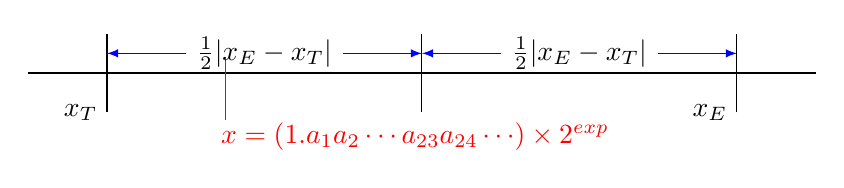
\begin{tikzpicture}
%\usetikzlibrary{shapes.multipart}
\draw(0,0) -- (10,0);
\draw[red](2.5,-0.6) node[below=6pt,right=-5pt]{$x=(1.a_1a_2\cdots a_{23}a_{24}\cdots)\times2^{\text{exp}}$}-- (2.5,0.2) ;
\draw(1,-0.5) node[anchor=east]{$x_T$}--(1,0.5) ;
\draw(9,-0.5) node[anchor=east]{$x_E$}--(9,0.5);
\draw(5,-0.5)--(5,0.5);
\draw[blue,latex-](1,0.25)--(2,0.25);
\draw[blue, -latex](4,0.25)--(5,0.25);
\draw[blue, latex-](5,0.25)--(6,0.25);
\draw[blue, -latex](8,0.25)--(9,0.25);
\draw(3,0.25)node{$\frac{1}{2}\vert x_E-x_T\vert$ };
\draw(7,0.25)node{$\frac{1}{2}\vert x_E-x_T\vert$};


\end{tikzpicture}
\caption{Posición relativa de un número no máquina $x$ y su redondeo a número máquina por truncamiento $x_T$ y por exceso $x_E$ Si redondeamos al más próximo de los dos, el error es siempre menor o igual a la mitad del intervalo $x_E-x_T$.}
\label{fig:errorred}
\end{figure} 

Examinando con un poco de detalle el resultado anterior, vemos que consta de tres términos. El término $\frac{1}{2}$ surge de aproximar un número real por su número máquina más cercano, El termino $2^\text{exp}$ depende del tamaño del número. Para números grandes este factor será grande y para números pequeños será un factor pequeño. Por último queda el factor $2^{-23}$;  este factor está directamente relacionado con la mantisa empleada en la representación. Efectivamente, si hubiéramos  representado el número en el estándar de doble precisión, es fácil demostrar que el error absoluto cometido habría quedado acotado como,

 \begin{equation*}
\vert x-x_r \vert \leq \frac{1}{2}\vert x_E-x_T \vert= \frac{1}{2}\cdot 2^{-52}\cdot 2^\text{exp}
\end{equation*}
 
\index{epsilon del computador} Es decir, el único factor que cambia en el error es precisamente el término relacionado con el tamaño de la mantisa. Este término recibe el nombre de precision del computador o \emph{epsilon del computador} (eps). Y vale siempre 2 elevado a menos ($-$) el  número de bits de la mantisa. Por tanto, podemos generalizar la expresión parar la cota del error absoluto como,

  \begin{equation*}
\vert x-x_r \vert \leq \frac{1}{2}\vert x_E-x_T \vert= \frac{1}{2}\cdot\ \text{eps}\cdot2^\text{exp}
\end{equation*}

El significado del \emph{epsilon} del computador queda aún más claro si definimos el error relativo..

\begin{equation*}
\text{Error relativo}=\frac{\vert x-x_r \vert}{\vert x \vert} \leq \frac{1}{2}\frac{\vert x_E-x_T \vert}{\vert x \vert}= \frac{1}{2}\cdot \frac{\text{eps}\cdot2^\text{exp}}{(1.a_1a_2\cdots a_{23}a_{24}\cdots)\times2^{\text{exp}}}\leq \frac{1}{2}\text{eps}
\end{equation*}

El error relativo pondera el valor del error cometido con la magnitud del número representado.  Un ejemplo sencillo ayudará a entender mejor su significado. Imaginemos que tuviéramos un sistema de representación que solo nos permitiera representar número enteros. Si queremos representar los números $1.5$ y $1000000.5$ su representación sería $1$ y $1000000$ en ambos casos hemos cometido un error absoluto de 0.5. Sin embargo si comparamos con los números representados, en el primer caso el error vale la mitad del número mientras que en el segundo no llega a una millonésima parte.

En el caso de la representación que estamos estudiando, el error relativo cometido para cualquier número representable es siempre más pequeño que la mitad del \emph{epsilon} del computador,


\begin{equation*}
x_r=x\cdot (1+ \delta); | \delta| \leq \frac{1}{2}\cdot eps
\end{equation*}


Un último comentario sobre el \emph{epsilon} del computador, entendido como precisión. La diferencia entre dos números máquina consecutivos está estrechamente  relacionada con el \emph{epsilon}. Si tenemos un número máquina y queremos incrementarlo en la cantidad más pequeña posible, dicha cantidad es precisamente el \emph{epsilon}, multiplicado por 2 elevado al exponente del número. La razón de que esto sea así está relacionada con el modo en que se suman dos números en la representación en punto flotante. Supongamos que tenemos un número cualquiera representado en el estándar de precisión simple,

\begin{tabular}{|c||c||c|}
\hline
sig.&$\leftarrow$mantisa, 23 bits $\rightarrow$&$\leftarrow$ exponente, 8 bits $\rightarrow$\\
\hline
0&11110000000000000000000&10000000\\
\hline
\end{tabular}\\

El número representado tiene de exponente $2^7-127=1$. Supongamos ahora que quisieramos sumar a este número la cantidad $2^{-22}$ su representación en el estándar emplearía una mantisa de ceros (recordar el 1 ímplicito) y un exponente $-22+127=105$. Sería por tanto,

\begin{tabular}{|c||c||c|}
\hline
sig.&$\leftarrow$mantisa, 23 bits $\rightarrow$&$\leftarrow$ exponente, 8 bits $\rightarrow$\\
\hline
0&00000000000000000000000&01101001\\
\hline
\end{tabular}\\

Para sumar dos números en notación científica es imprescindible que los dos estén representados con el mismo exponente, para entonces poder sumar directamente las mantisas. Disminuir el exponente del mayor de ellos hasta que coincida con el del menor no es posible, ya que eso supondría añadir dígitos a la parte entera de la mantisa, pero no hay bits disponibles para ello entre los asignados a la mantisa. Por tanto, la solución es aumentar el exponente del menor de los números, hasta que alcance el valor del exponente del mayor, y disminuir el valor de la mantisa desnormalizándola, es decir sin considerar el 1 implícito. 
Por tanto en nuestro ejemplo, debemos representar $2^{-22}$ empleando un exponente 1, $2^{-22}\rightarrow 2^{-23}\cdot 2^1$,

\begin{tabular}{|c||c||c|}
\hline
sig.&$\leftarrow$mantisa \textbf{(desnorm.)}, 23 bits $\rightarrow$&$\leftarrow$ exponente, 8 bits $\rightarrow$\\
\hline
0&00000000000000000000001&100000000\\
\hline
\end{tabular}\\

La suma de ambos números se obtiene sumando directamente las mantisas,

\begin{tabular}{|c||c||c|}
\hline
sig.&$\leftarrow$mantisa, 23 bits $\rightarrow$&$\leftarrow$ exponente, 8 bits $\rightarrow$\\
\hline
0&1111000000000000000000\textbf{1}&10000000\\
\hline
\end{tabular}\\

¿Qué pasa si tratamos de sumar un número más pequeño,por ejemplo $2^{-23}$? Al representarlo con exponente 1 para poder sumarlo el número tomaría la forma, $2^{-23}\rightarrow 2^{-24}\cdot2^{1}$. Es fácil ver el problema, con una mantisa de 23 bits nos se puede representar el número $2^{-24}$ porque ya no hay \emph{hueco} para él. La mantisa sería cero y --dado que se trata de una representación desnormalizada--, el número resultante sería cero. Por tanto, al sumarlo con el número inicial nos daría este mismo número.

Esto nos lleva a que la precisión del computador no es igual para todos los números representables, sino que depende de su magnitud. la precisión, tomada en función de la distancia entre dos números consecutivos, es: $\text{precisión}=\text{eps}\cdot 2^{exp}$ y su valor se duplica cada vez que aumentamos el exponente en una unidad. La figura \ref{fig:precision} muestra esquemáticamente este fenómeno.
\begin{figure}[h]
	\centering
		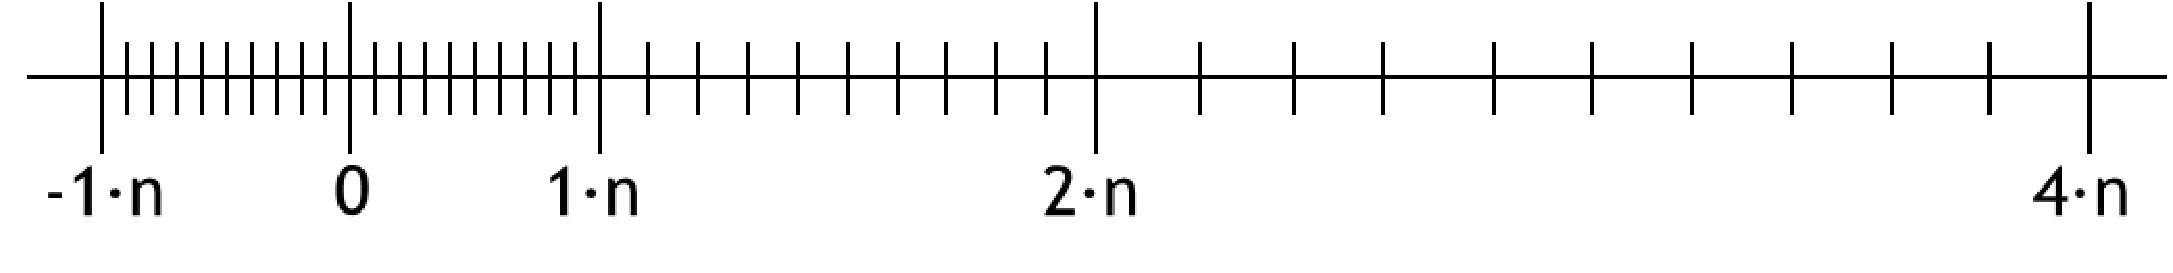
\includegraphics[width=10cm]{precision.pdf}
	\caption{Ilustración del cambio de precisión con la magnitud de los números representados.}
	\label{fig:precision}
\end{figure}

\subsection{Errores de desbordamiento}\index{Desbordamiento}
En el apartado anterior hemos visto una de las limitaciones de la representación numérica de los ordenadores; el hecho de usar una mantisa finita hace que solo unos pocos números tengan representación exacta, el resto hay que aproximarlos cometiendo errores de redondeo. En este apartado nos centraremos en estudiar las limitaciones debidas al hecho de usar un exponente finito; solo podemos representar un rango limitado de valores.
La figura \ref{fig:desbord} muestra esquemáticamente el rango de números representables. El número negativo más pequeño representable, viene definido, por un bit de signo 1, para indicar que se trata de un número negativo y la mantisa y el exponente más grandes que, dentro de las especificaciones del estándar, todavía representan un número finito. Cualquier número negativo menor que éste, produce un error de desbordamiento conocido en la literatura técnica con el nombre de \emph{overflow} negativo. El número negativo más próximo a cero, que se puede representar será aquel que tenga bit de signo 1, la mantisa (desnormalizada) más pequeña posible y el exponente más pequeño posible. Cualquier número más próximo a cero que este, será representado por el ordenador como cero. Se ha producido en este caso un error de desbordamiento conocido como \emph{underflow} negativo. 

De modo análogo a como hemos definido el número negativo más pequeño representable, podemos definir el número positivo más grande representable. La única diferencia será que en este caso el bit de signo toma valor cero para indicar que es un  número positivo. Cualquier número mayor que éste que queramos representar, provocará un error de desbordamiento (\emph{overflow} positivo.) Por último, el número positivo más próximo a cero representable coincide con el correspondiente negativo, de nuevo salvo en el bit de signo, que ahora deberá ser cero. En el caso de tratar de representar un número más pequeño el ordenador no lo distinguirá de cero, produciéndose un desbordamiento denominado \emph{underflow} positivo. 
\begin{figure}[h]
	\centering
		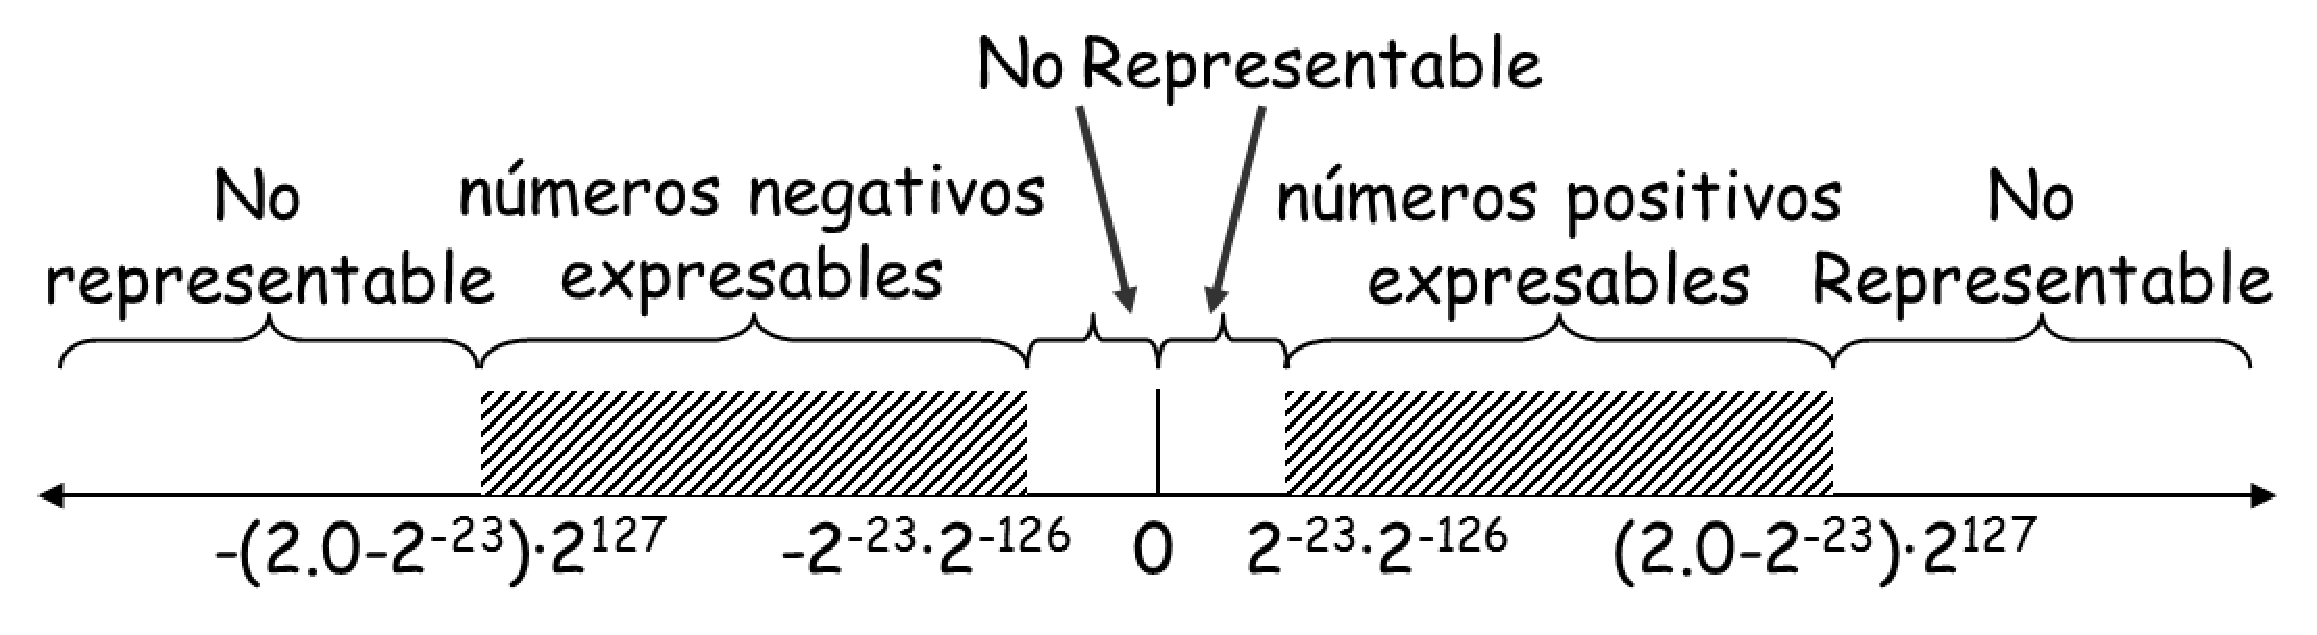
\includegraphics[width=10cm]{underandover.pdf}
	\caption{Números representables y desbordamientos en el estándar IEEE 754 de precisión simple.}	
	\label{fig:desbord}
\end{figure}

\section{Errores derivados de las operaciones aritméticas}\index{Errores aritméticos}
Hasta ahora, nos hemos centrado siempre en el problema de la representación numérica del computador. En esta sección vamos a introducir un nuevo tipo de errores que tienen si cabe todavía más importancia desde el punto de vista del cálculo científico. Se trata de los errores derivados de las operaciones aritméticas.

Indirectamente ya se introdujo el problema en la sección anterior al hablar de la precisión del computador, y de la necesidad de igualar los exponentes de los sumandos al mayor de ellos antes de poder sumar en formato de punto flotante. Veamos en más detalle algunas consecuencias de la aritmética en punto flotante.
\subsection{Acumulación de errores de redondeo}\index{Acumulación de errores}

Para empezar, se ilustrará el proceso de la suma de dos números representados en base 10 en formato de punto flotante. Supongamos que queremos sumar los números $99.99$ y $0.161$. Supongamos además que seguimos una representación en punto flotante con las siguientes limitaciones la mantisa es de cuatro dígitos, el exponente es de dos dígitos.

Si sumamos los números, tal y como los hemos escrito más arriba, sin seguir formato de punto flotante, el resultado sería,

\begin{equation*}
99.99+0.161=100.151
\end{equation*}

Supongamos que los representamos ahora en el formato de punto flotante descrito más arriba, $99.99=9.999\times10^1$, $0.161=1.610\times10^{-1}$. Vamos a descomponer el proceso de sumar estos dos números en cuatro pasos, que reflejan, esquemáticamente, el proceso que seguiría un computador.

\begin{enumerate}
\item \textbf{Alineamiento.} \index{Alineamiento}Consiste en representar el número más pequeño empleando el exponente del mayor. Para ellos se desplazan hacia la derecha los dígitos del número más pequeño tantas posiciones como indique la diferencia de los exponentes de los dos números y se cambiar el exponente del número mas pequeño por el del más grande.
\begin{equation*}
1.610\times 10^{-1}\rightarrow 0.016\times10^1
\end{equation*}
Como cabía esperar, el desplazamiento hacia la derecha de la mantisa produce la pérdida de los últimos dígitos del número. Tenemos aquí un primer error de redondeo en el proceso de alineamiento.

\item \textbf{Operación.}
Una vez que los operandos están alineados, se puede realizar la operación. Si la operación es suma y los signos son iguales o si la operación es resta y los signos son diferentes, se suman las mantisa. En otro caso se restan.

Es importante comprobar tras realizar la operación si se ha producido desbordamiento de la mantisa; en el ejemplo propuesto:

\begin{tabular}{c r}
&$9.999\cdot10^1$\\
$+$&$0.016\cdot10^1$\\
\hline
&$10.015\cdot10^1$
\end{tabular}\\

No es posible emplear directamente el resultado de la suma de las mantisas de los sumandos como mantisa de la suma ya que requeriría emplear un dígito más. El resultado obtenido desborda el tamaño de la mantisa.

\item \textbf{Normalización.}
Si se ha producido desbordamiento de la mantisa, es preciso volver a normalizarla,
\begin{equation*}
10.015\times10^1=1.0015\times10^2
\end{equation*}
 
\item \textbf{Redondeo.} El desplazamiento de la mantisa hace que no quepan todo los dígitos, por lo que es necesario redondearla (por truncamiento o por exceso),

\begin{equation*}
1.0015\times10^2=1.002\times10^2
\end{equation*}

Por último, se comprueba si las operaciones realizadas han producido desbordamiento del exponente, en cuyo caso el resultado sería un número no representable: $\infty$ ó $0$.

\item \textbf{Renormalización} Para números en representación binaria es preciso a veces volver a normalizar la mantisa después del redondeo. Supongamos, como en el ejemplo anterior, una mantisa de cuatro bits, ---ahora con números representados en binario--- y que tras realizar una operación suma el resultado que se obtiene es $11.111\times2^1$. La mantisa ha desbordado y hay que normalizarla $11.111\times2^1\rightarrow1.1111\times2^2$. Tenemos que redondear la mantisa y lo normal en este caso dado que el número estaría exactamente en la mitad del intervalo entre dos números representables, es hacerlo por exceso: $1.1111\times2^2\rightarrow10.000\times2^2$. la operación de redondeo por exceso ha vuelto a desbordar la mantisa y, por tanto, hay que volver a normalizarla: $10.000\times2^2\rightarrow1.000\times2^3$.
\end{enumerate} 

Analicemos el error cometido para la suma empleada en los ejemplos anteriores. En aritmética exacta, el número obtenido tras la suma es $100.152$. Empleando la representación en punto flotante, con una mantisa de cuatro dígitos el resultado es $1.002\times10^2=100.2$. por tanto, el error absoluto cometido es,
\begin{equation*}
\vert 100.151-100.2 \vert=0.049
\end{equation*}

y el error relativo,
\begin{equation*}
\left\vert\frac{100.151-100.2 }{100.152}\right\vert\approx 0.000489
\end{equation*}
En general puede comprobarse que para cualquier operación aritmética básica $\odot \ $(suma, resta, multiplicación división) y dos números máquina $x$, $y$ se cumple,

\begin{equation*}
\text{flotante}(x\odot y)=(x\odot y)\cdot(1+\delta) \ \ \vert \delta \vert \leq eps
\end{equation*}

Este enunciado se conoce como el axioma fundamental de la aritmética en punto flotante:\emph{ El eps del computador es la cota superior del error relativo en cualquier operación aritmética básica realizada en punto flotante entre números máquina.} 

El axioma fundamental de la aritmética en punto flotante establece una cota superior para el error. En la práctica, es frecuente que se encadenen un gran número de operaciones aritméticas elementales. Al encadenar operaciones, los errores cometidos en cada una de ellas se acumulan.

Supongamos por ejemplo que queremos realizar la operación $x\cdot(y+z)$ en aritmética flotante la operación podríamos describirla como,
\begin{align*}
\text{flotante}\left(x\cdot (y+z)\right)& =\left(x\cdot\text{flotante}(y+z)\right)\cdot(1+\delta_1)\\
 & = (x\cdot(y+z))\cdot(1+\delta_2)\cdot(1+\delta_1)\\
 & \approx (x\cdot(y+z))\cdot(1+2\delta)
\end{align*}

Donde $\delta_1$ representa el error relativo cometido en el producto y $\delta_2$ el error relativo cometido en la suma. Ambos errores están acotados por el \emph{eps} del ordenador ($\delta_1, \ \delta_2 \leq eps$). El valor $\delta$ se puede obtener como,
\begin{equation*}
(1+\delta_1)\cdot(1+\delta_2)=1+\delta_1\delta_2+\delta_1+\delta_2\approx 1+2\delta,\ \delta=\max(\delta_1,\delta_2)
\end{equation*}

Podemos concluir que, en este caso, el error de redondeo relativo duplica al de una operación aritmética sencilla. En general, el error tenderá a multiplicarse con el número de operaciones aritméticas encadenadas.

Hay situaciones en las cuales los errores de redondeo que se producen durante una operación aritmética son considerables por ejemplo, cuando se suman cantidades grandes con cantidades pequeñas,

\begin{equation*}
\text{flotante}(1.5\cdot10^{38}+1.0\cdot10^0)=1.5\cdot10^{38} + 0
\end{equation*}

En este caso, durante el proceso de alineamiento, es preciso desplazar la mantisa del número pequeño 38 posiciones decimales para poder sumarlo. Con cualquier mantisa que tenga menos de 38 dígitos el resultado es equivalente a convertir el segundo sumando en cero.

Otro ejemplo es la pérdida de la propiedad asociativa,

\begin{equation*}
\left. \begin{aligned}
x=1.5\cdot10^{38}\\
y=-1.5\cdot10^{38}\\
\end{aligned}
\right\}
\Rightarrow
(x+y)+1\neq x+(y+1)
\begin{cases}
(x+y)+1=1\\
x+(y+1)=0
\end{cases}
\end{equation*}

Los resultados pueden estar sometidos a errores muy grandes cuando la operación aritmética es la sustracción de cantidades muy parecidas. Si, por ejemplo, queremos realizar la operación $100.1-99.35=0.75$ y suponemos que estamos empleando una representación en punto flotante con una mantisa de cuatro dígitos y los números representados en base 10 ($100.1=1.001\cdot10^2$, $99.35=9.935\cdot 10^1$) 

\begin{enumerate}
\item \textbf{Alineamiento}
\begin{equation*}
9.935\cdot 10^1\rightarrow 0.994 \cdot 10^2
\end{equation*}

\item \textbf{Operación}

\begin{tabular}{c r}
&$1.001\cdot10^2$\\
$-$&$0.994\cdot10^2$\\
\hline
&$0.007\cdot10^2$
\end{tabular}\\

\item \textbf{normalización}
\begin{equation*}
0.007\cdot10^2\rightarrow 7.000\cdot10^{-1}
\end{equation*}
\end{enumerate}

Los pasos $4$ y $5$ no son necesarios en este ejemplo. Si calculamos ahora el error absoluto de redondeo cometido,
\begin{equation*}
\vert 0.75-0.7 \vert =0.05
\end{equation*} 

Y el error relativo,
\begin{equation*}
\left\vert\frac{0.75-0.7}{0.75}\right\vert\approx 0.0666
\end{equation*}
Es decir, se comete un error de un $6,7\%$. El problema en este caso surge porque en el proceso de alineamiento perdemos un dígito significativo.

 En un sistema de representación en punto flotante en que los números se representan en base $\beta$ y el tamaño de la mantisa es $p$, Si las sustracciones se realizan empleando $p$ dígitos, el error de redondeo relativo puede llegar a ser $\beta-1$.
 
Veamos un ejemplo para números en base 10 ($\beta=10$). Supongamos que empleamos una mantisa de cuatro dígitos y que queremos realizar la operación $1.000\cdot10^0-9.999\cdot10^{-1}$. El resultado exacto sería, $1-0.9999=0.0001$. Sin embargo, en el proceso de alineamiento,
\begin{equation*}
9.999\cdot10^{-1}\rightarrow0.9999\cdot10^0
\end{equation*} 
Si redondeamos el número por exceso, el resultado de la sustracción sería cero. Si lo redondeamos por defecto,

\begin{tabular}{c r}
&$1.000\cdot10^0$\\
$-$&$0.999\cdot10^0$\\
\hline
&$0.001\cdot10^0$
\end{tabular}\\

y el error relativo cometido sería,
\begin{equation*}
\left\vert\frac{1.000\cdot10^{-4}-1.000\cdot10^{-3}}{1.000\cdot10^{-4}}\right\vert=\frac{10^{-4}(10-1)}{10^{-4}}=10-1\Rightarrow\beta -1
\end{equation*}


Para paliar estos problemas, el estándar IEEE 754 establece que las operaciones aritméticas deben realizarse siempre empleando dos dígitos extra para guardar los resultados intermedios. Estos dos dígitos extra reciben el nombre de dígitos de protección o dígitos de guarda (\emph{guard digits}).
Si repetimos la sustracción, $100.1-99.35$, empleando los dos dígitos de guarda,

\begin{enumerate}
\item \textbf{Alineamiento}
\begin{equation*}
9.935{\color{red}00}\cdot=10^1\rightarrow 0.993{\color{red}50} \cdot 10^2
\end{equation*}

\item \textbf{Operación}
\begin{tabular}{c r}
&$1.001{\color{red}00} \cdot10^2$\\
$-$&$0.993{\color{red}50}\cdot10^2$\\
\hline
&$0.007{\color{red}50}\cdot10^2$
\end{tabular}\\

\item \textbf{normalización}
\begin{equation*}
0.007{\color{red}50}\cdot10^2\rightarrow 7.500\cdot10^{-1}
\end{equation*}

\end{enumerate}
En este caso, obtenemos el resultado exacto. En general, empleando dos bits de guarda para realizar las sustracciones el error de redondeo es siempre menor que el \emph{eps} del computador.


\subsection{Anulación catastrófica}\index{Anulación catastrófica}
La anulación catastrófica se produce cuando en una operación aritmética, típicamente la sustracción,  los dígitos más significativos de los operandos, que no están afectados por el redondeo, se cancelan entre sí. El resultado contendrá fundamentalmente dígitos que sí están afectados por errores de redondeo. Veamos un ejemplo,

Supongamos que queremos realizar la operación $b^2-4\cdot a \cdot c$ empleando números en base 10, y una mantisa de 5 dígitos. Supongamos que los números empleados son: $b= 3.3357\cdot10^0$, $a=1.2200\cdot10^0$, $c=2.2800\cdot10^0$. El resultado exacto de la operación es,
\begin{equation}
b^2-4\cdot a\cdot c=4.944\cdot10^{-4}
\end{equation}

Si realizamos las operaciones en la representación pedida,
\begin{align*}
b^2=1.1126{\color{red}89}\cdot10^1\\
4\cdot a\cdot c=1.1126{\color{red}40}\cdot10^1\\
b^2-4\cdot a\cdot c=5.0000\cdot10^{-4}
\end{align*}

El error relativo cometido es aproximadamente un 1\%. Como se han utilizado dos bits de guarda en las operaciones intermedias, la sustracción no comente en este caso error alguno. El error se debe a los redondeos de los resultados anteriores. Una vez realizada la sustracción, el resultado solo contiene los dígitos sometidos a redondeo ya que los anteriores se han anulado en la operación.

Como regla práctica se debe evitar al realizar operaciones aritméticas aquellas situaciones en las que se sustraen cantidades casi iguales. Veamos otro ejemplo, para ilustrar esta idea. Supongamos que queremos realizar la operación,
\begin{equation*}
y=\sqrt{x^2+1}-1
\end{equation*}
Para valores pequeños de $x$, esta operación implica una anulación con pérdida de dígitos significativos. Una posible solución es utilizar una forma alternativa de construir la ecuación. Si multiplicamos y dividimos por el conjugado,

\begin{equation*}
y=(\sqrt{x^2+1}-1)\cdot\left(\frac{\sqrt{x^2+1}+1}{\sqrt{x^2+1}+1}\right)=\frac{x^2}{\sqrt{x^2+1}+1}
\end{equation*}

\subsection{Errores de desbordamiento}

Al, hablar del rango finito de los números representables, se indicó cómo trata el éstandar IEEE 754 los números que desbordan los límites de representación. Al realizar operaciones aritméticas, es posibles llegar a situaciones en las que el resultado sea un número no representable bien por se demasiado grande en magnitud, (\emph{Overflow} positivo o negativo) o por ser demasiado pequeño, (\emph{underflow} positivo o negativo.) Un ejemplo que nos permite ilustrar este fenómeno es el del cálculo del módulo de un vector,

\begin{equation*}
\vert\vert\vec{v}\vert\vert=\vert\vert(v_1, v_2\cdots v_n\vert\vert=\sqrt{\sum_{i=1}^nv_i^2}
\end{equation*}

Supongamos que creamos el siguiente programa en Matlab para calcular el módulo de un vector

% \begin{lstlisting}
% function m=norma(x)
% %inicializamos a cero la variable que contendrá la norma del vector.
% m=0;
% n=length(x) %calculamos la longitud del vector.
% %creamos un bucle para ir sumando los cuadrados de las componentes
% for i=1:n
% m=m+x(i)^2;
% end

% %calculamos la raíz cuadrada del resultado del bucle
% m=sqrt(m)
% \end{lstlisting}

El programa anterior provocará un error de desbordamiento incluso para n=1, si introducimos un número cuyo cuadrado sea mayor que el mayor número representable. Por ejemplo si introducimos el número, $ 2^{1024/2}=1.340780792994260e+154$ en nuestro programa Matlab devolverá como solución \emph{inf}. Es decir, el resultado produce un error de desbordamiento. El problema se produce en el bucle, al calcular el cuadrado del número,
\begin{equation*}
\left(2^{1024/2}\right)^2=2^{1024}> (2-2^{-52})\cdot 2^{1023}
\end{equation*}

Una vez producido el desbordamiento el resto de las operaciones quedan invalidadas. Como en casos anteriores, la solución a este tipo de problemas exige modificar la forma en que se realizan los cálculos. Un primer paso sería igualar el módulo al valor absoluto del número cuando n=1. De este modo, el modulo del número propuesto en el ejemplo anterior se podría calcular correctamente.

Todavía es posible mejorar el programa, y ampliar el rango de vectores para los que es posible calcular el módulo. Para ello es suficiente recurrir a un pequeño artificio: dividir los elementos del vector por el elemento de mayor tamaño en valor absoluto, calcular el módulo del vector resultante, y multiplicar el resultado de nuevo por el elemento de mayor tamaño,
\begin{align*}
\sqrt{\sum_{i=1}^nv_i^2}=\vert\max{v_i}\vert\cdot\sqrt{\sum_{i=1}^n\left(\frac{v_i}{\vert\max{v_i}\vert}\right)^2}
\end{align*}

El siguiente código permite calcular el módulo de un vector usando este procedimiento\footnote{El programa no funcionará correctamente para vectores cuyos primeros elementos sean 0, $(0,0,0\cdots$},

% \begin{lstlisting}
% function m=norma(x)
% n=length(x); %calculamos la longitud del vector.
% %si n=1 nos limitamos a devolver el valor absoluto del número introducido
% if n==1
% 	x=abs(x);
% else
% % inicializamos con el primer elemento la variable que contendrá
% % al mayor de los elementos del vector
% mayor=abs(x(1));

% % inicialimos a 1 la variable que contendrá la suma de
% % los cuadrados de los elementos divididos por el valor de ello

% nscalado=1

% % creamos un bucle para ir sumando los cuadrados de las componentes.
% % empezamos en el segundo elemento, puesto que el primero ya lo tenemos.
% 	for i=2:n	
% 		% calculamos el valor absoluto del elemento i
% 		modxi=abs(x(i))
% 		% comparamos con modxi con el mayor elemento obtenido hasta
% 		% aquí
% 		if mayor<modxi
% 			% si modxi es mayor, será el elemento más grande encontrado
% 			% hasta esta iteración
% 			% cambiamos el valor de la suma 
% 			mscalado=1+mscalado*(modxi/mayor)^2;
% 			% definimos mayor como el nuevo valor encontrado
% 			mayor=modxi;
% 		else
% 			% si no es el más grande, nos limitamos a sumarlo al resto
% 			mscalado=mscalado+(modxi/mayor)^2;
	
% 		end
% % una vez completado el bucle que calcula la suma de cuadrados,
% % obtenemos la raíz cuadrada, y multiplicamos por el mayor.
% m=mayor*sqrt(mscalado)
% \end{lstlisting}

Si aplicamos este programa a obtener la norma del vector,
\begin{equation*}
x=[2^{1024/2}\ 2^{1024/2}]
\end{equation*}
obtenemos como resultado,
\begin{equation*}
m=1.896150381621836\cdot10^{154}
\end{equation*}
En lugar de un error de desbordamiento (\emph{inf}).



  	 